Un ayuntamiento es responsable de mantener la siguiente red de carreteras. El número en cada arista es la longitud de la carretera en kilómetros.

\vspace{0.5cm} % Espacio vertical para separar el texto del gráfico

\begin{center}
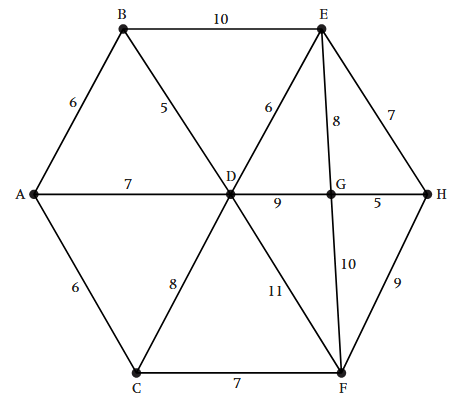
\includegraphics{ejercicios/carreteras_estado.png}

\end{center}

\vspace{0.5cm} % Espacio vertical

La oficina del ayuntamiento está ubicada en A.

\textbf{(a)} Un trabajador del ayuntamiento tiene que inspeccionar todas las carreteras, empezando y terminando en A. Encuentre la longitud de una ruta óptima.

\vspace{0.5cm} 

\textbf{(b)} Un supervisor, con base en A, también desea inspeccionar todas las carreteras. Sin embargo, el supervisor vive en H y desea comenzar su ruta en A y terminar en H. Encuentre la longitud de una ruta óptima para el supervisor.

\vspace{0.5cm}
\textbf{Solución}
\vspace{0.5cm}

\textbf{(a)} Hay cuatro vértices de grado impar: A, B, C y H.
Hay tres formas de emparejar estos vértices impares y la longitud mínima de cada emparejamiento es:
\begin{align*}
\text{AB + CH} &= 6 + 16 = 22 \\
\text{AC + BH} &= 6 + 17 = 23 \\
\text{AH + BC} &= 21 + 12 = 33
\end{align*}

La longitud de todas las carreteras en la red es 116.
La longitud de una ruta óptima del cartero chino para el trabajador es $116 + 22 = 138$ kilómetros.

\vspace{1cm} 

\textbf{(b)} Comenzar en A y terminar en H deja dos vértices de grado impar: B y C (que hay que unir).
La distancia mínima de B a C es 12.
Si empieza el camino en A acabará en H con una distancia de $116 + 12 = 128$ kilómetros.